% Last Update: $Id$
\section{Der Paketfilter (IPv4)}
\configlabel{PF\_NEW\_CONFIG}{PFNEWCONFIG}

\newcommand{\fwaction}[1]{{\small\textsf{#1}}}
\newcommand{\fwchain}[1]{\texttt{#1}}
\newcommand{\fwtable}[1]{\textsc{#1}}
\newcommand{\fwmatch}[1]{\texttt{#1}}
\newcommand{\fwpktstate}[1]{\texttt{#1}}
\newcommand{\fwloglevel}[1]{\texttt{#1}}
\newcommand{\protocol}[1]{\texttt{#1}}
\newcommand{\host}[1]{\texttt{#1}}
\newcommand{\package}[1]{\texttt{#1}}

Der von fli4l verwendete Linux-Kern stellt einen Paketfilter zur
Verfügung. Mit Hilfe dieses Paketfilters wird gesteuert, wer mit dem
Router bzw. über ihn hinweg kommunizieren darf. Weiterhin können
Dinge wie Port-Weiterleitung (ein an den Router gerichtetes Paket wird
an einen anderen internen Rechner weitergereicht) und Maskierung
(engl. ``Masquerading''; Pakete, die von einem Rechner hinter dem Router
kommen, werden so verändert, dass sie so aussehen, als kämen sie vom Router
selbst) realisiert werden.

Die Struktur des Paketfilters ist in Abbildung \ref{fig:netfilter}
angedeutet. Pakete kommen über eine Netzwerk-Schnittstelle herein und
durchlaufen die \fwchain{PREROUTING}-Kette (eng. ``chain''). Hier werden die an
den Router gerichteten Pakete an einen anderen Rechner weitergereicht, indem die
Zieladresse und der Zielport manipuliert werden. Ist das Paket
an den Router gerichtet, wird es an die \fwchain{INPUT}-Kette, andernfalls an
die \fwchain{FORWARD}-Kette weitergereicht. Beide Ketten prüfen, ob das Paket
zulässig ist. Wird das Paket akzeptiert, wird es an den lokalen
Zielprozess zugestellt oder über die \fwchain{POSTROUTING}-Kette (in der das
Maskieren von Paketen stattfindet) an diejenige Netzwerk-Schnittstelle
weitergereicht, über die das Paket sein Ziel erreichen kann. Lokal generierte
Pakete werden in der \fwchain{OUTPUT}-Kette gefiltert und schließlich (falls
erfolgreich) über die \fwchain{POSTROUTING}-Kette ebenfalls an die korrekte
Netzwerk-Schnittstelle weitergereicht.

\begin{figure}[htbp]
  \centering
  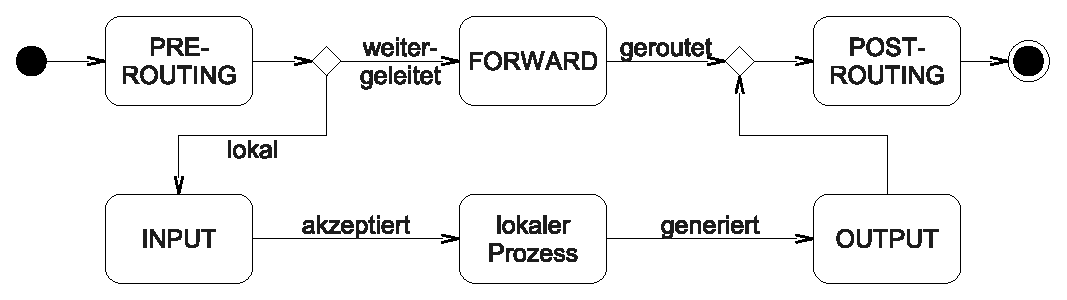
\includegraphics[width=\columnwidth]{firewall}
  \caption{Struktur des Paketfilters}
  \label{fig:netfilter}
\end{figure}

Mit der Paketfilterkonfiguration lassen sich die einzelnen
Ketten des Paketfilters direkt konfigurieren. Dazu gibt es für
jede relevante Kette ein eigenes Array, d.h. eine für die
\fwchain{INPUT}-Kette (\var{PF\_INPUT\_\%}), eine für die
\fwchain{FORWARD}-Kette (\var{PF\_FORWARD\_\%}), eine für die
\fwchain{OUTPUT}-Kette (\var{PF\_OUTPUT\_\%}), eine für die
\fwchain{PREROUTING}-Kette, in der die Portweiterleitung durchgeführt wird
(\var{PF\_PREROUTING\_\%}), und eine für die \fwchain{POSTROUTING}-Kette,
in der das Maskieren der Pakete durchgeführt wird (\var{PF\_POSTROUTING\_\%}).

Ein Eintrag in einem dieser Arrays besteht im
Wesentlichen aus einer Aktion (s.u.),
die durch zusätzliche Bedingungen eingeschränkt werden kann. Diese Bedingungen
beziehen sich auf Eigenschaften des betrachteten Paketes. Ein Paket
enthält Informationen über seine Herkunft (Quelle, welcher Rechner hat
das Paket losgeschickt), sein Ziel (an welchen Rechner und welche
Anwendung soll das Paket gehen) u.a.m. Bedingungen können sich auf
folgende Eigenschaften eines Paketes beziehen:

\begin{itemize}
  \item die Quelle (Quell-Adresse, Quell-Port oder beides)
  \item das Ziel (Ziel-Adresse, Ziel-Port oder beides)
  \item das Protokoll
  \item die Schnittstelle, über welches das Paket hereinkommt bzw. hinausgeht
  \item die MAC-Adresse des Rechners, von dem das Paket kommt
  \item den Zustand des Paketes bzw. der Verbindung, zu der das Paket gehört
\end{itemize}

Kommt ein Paket herein, werden die Einträge bzw. die daraus generierten
Regeln von oben nach unten abgearbeitet und die erste Aktion
ausgeführt, bei der alle Bedingungen gelten.  Trifft keine der Regeln
zu, wird die Standardaktion ausgeführt, die man für (fast) jede
Tabelle angeben kann.

Ein Eintrag hat dabei folgendes Format, wobei zu beachten ist, dass
alle Einschränkungen optional sind:

\begin{example}
\begin{verbatim}
    restriction{0,} [[source] [destination]] action [BIDIRECTIONAL|LOG|NOLOG]
\end{verbatim}
\end{example}

An allen Stellen, an denen Netzwerke, IP-Adressen oder Hosts angegeben werden
müssen, kann man sich auch auf \var{IP\_NET\_\%}, \var{IP\_NET\_\%\_IPADDR} oder
via \host{@hostname} auf einen Host aus \var{HOST\_\%} beziehen. Ist
\var{OPT\_DNS} aktiviert, dann können außerhalb von Aktionen via \host{@fqdn}
auch Hosts über ihren Namen referenziert werden, die \emph{nicht} in
\var{HOST\_\%} zu finden sind. Das ist insbesondere dann sinnvoll, wenn es
sich um externe Hosts handelt, die zudem viele (und wechselnde) IP-Adressen
besitzen.

\marklabel{sec:fwrules_actions}{\subsection{Aktionen des Paketfilters}}

Aktionen können die folgenden sein:
\begin{center}
    \begin{longtable}{|l|l|p{0.5\textwidth}|}
        \hline
        \multicolumn{1}{|l}{\textbf{Aktion}} &
        \multicolumn{1}{|l}{\textbf{Kette(n)}} &
        \multicolumn{1}{|l|}{\textbf{Bedeutung}} \\
        \hline
        \endhead
        \hline
        \endfoot
        \endlastfoot
        \fwaction{ACCEPT}       & alle
                                & Akzeptiere das Paket.
                                \\
        \hline
        \fwaction{DROP}         &
                                \begin{tabular}[t]{@{}l@{}}
                                    \fwchain{INPUT} \\
                                    \fwchain{FORWARD} \\
                                    \fwchain{OUTPUT}
                                \end{tabular}
                                & Verwirf das Paket (der Absender erkennt das
                                nur daran, dass keine Antwort, aber auch keine
                                Fehlermeldung zurückkommt).
                                \\
        \hline
        \fwaction{REJECT}       &
                                \begin{tabular}[t]{@{}l@{}}
                                    \fwchain{INPUT} \\
                                    \fwchain{FORWARD} \\
                                    \fwchain{OUTPUT}
                                \end{tabular}
                                & Weise das Paket zurück (der Absender erhält
                                eine entsprechende Fehlermeldung).
                                \\
        \hline
        \fwaction{LOG}          & alle
                                & Protokolliere das Paket und gehe zur nächsten
                                Regel. Um verschiedene Protokoll-Einträge
                                auseinanderhalten zu können, kann ein Präfix
                                verwendet werden, das via
                                \fwaction{LOG:log-prefix} angegeben wird. Dieses
                                Präfix darf maximal 28 Zeichen lang sein und
                                kann aus Buchstaben, Ziffern, dem Bindestrich
                                (\texttt{-}) und dem Unterstrich (\texttt{\_})
                                bestehen.
                                \\
        \hline
        \fwaction{MASQUERADE}   & \fwchain{POSTROUTING}
                                & Maskiere das Paket: Ersetze die Quelladresse
                                des Paketes durch die eigene, der Schnittstelle
                                zugewiesenen Adresse und sorge dafür, dass
                                Antworten für diese Verbindung an den richtigen
                                Rechner weitergeleitet werden.
                                \\
        \hline
        \fwaction{SNAT}         & \fwchain{POSTROUTING}
                                & Ersetze die Quelladresse und den Quellport
                                des Paketes durch die als Parameter für
                                \fwaction{SNAT} angegebene Adresse (für alle
                                Pakete, die zu der gerade betrachteten
                                Verbindung gehören).
                                \\
        \hline
        \fwaction{DNAT}         & \fwchain{PREROUTING}
                                & Ersetze die Zieladresse und den Zielport des
                                Paketes durch die als Parameter für
                                \fwaction{DNAT} angegebene Adresse (für alle
                                Pakete, die zu der gerade betrachteten
                                Verbindung gehören).
                                \\
        \hline
        \fwaction{REDIRECT}     &
                                \begin{tabular}[t]{@{}l@{}}
                                    \fwchain{PREROUTING} \\
                                    \fwchain{OUTPUT}
                                \end{tabular}
                                & Ersetze den Zielport des Paketes durch den
                                als Parameter für \fwaction{REDIRECT}
                                angegebenen Port und stelle das Paket lokal zu
                                (für alle Pakete, die zu der gerade
                                betrachteten Verbindung gehören).
                                \\
        \hline
        \fwaction{NETMAP}       &
                                \begin{tabular}[t]{@{}l@{}}
                                    \fwchain{PREROUTING} \\
                                    \fwchain{POSTROUTING}
                                \end{tabular}
                                & Bilde die Ziel- bzw. Quelladresse des Paketes
                                in den als Parameter für \fwaction{NETMAP}
                                angegebenen Bereich ab, die Ports bleiben
                                unverändert (für alle Pakete, die zu der gerade
                                betrachteten Verbindung gehören; in der
                                \fwchain{PREROUTING}-Kette wird die Zieladresse
                                verändert, in der \fwchain{POSTROUTING}-Kette
                                die Quelladresse).
                                \\
        \hline
        \caption{Aktionen in Paketfilterregeln}\marklabel{fwrule:actions}{}
    \end{longtable}
\end{center}

Einige dieser Aktionen können durch die Optionen \fwaction{BIDIRECTIONAL},
\fwaction{LOG} oder \fwaction{NOLOG} in ihrem Verhalten modifiziert werden.
\fwaction{BIDIRECTIONAL} generiert die gleiche Regel noch einmal, nur mit
vertauschter Quell- und Zieladresse (und vertauschtem Quell- und Zielport
und/oder vertauschter ein- und ausgehender Netzwerk-Schnittstelle, falls
angegeben). \fwaction{LOG}/\fwaction{NOLOG} aktivieren bzw. deaktivieren das
Protokollieren für diese eine Regel.

\marklabel{sec:fwrules_limits}{\subsection{Einschränkungen in den Regeln}}

Einschränkungen können durch die in den folgenden Abschnitten
aufgeführten Bedingungen vorgenommen werden. Bei den Bedingungen kann
man immer \fwmatch{any} angeben, wenn man an irgendeiner Stelle keine
Einschränkung vornehmen will, aber trotzdem etwas angeben
will/muss. Einschränkungen können in beliebiger Reihenfolge angegeben
werden, wenn sie einen vorangestellten Präfix haben. Das gilt für alle
Einschränkungen, außer für die Angabe einer Quell- bzw. Zieladresse. Diese
müssen immer direkt vor der Aktion stehen, die anderen Einschränkungen müssen
vorher erfolgen. Einschränkungen können auch negiert werden, dazu wird
einfach ein \fwmatch{!} vorangestellt.

\subsubsection{Einschränkungen der Quelle und des Ziels}

Jedes Paket enthält eine Quell- und eine Zielangabe, jeweils in Form
eines Tupels einer IP-Adresse und eines Ports.\footnote{Ein Port ist nur bei
TCP- und UDP-Paketen vorhanden.} Diese Quelle bzw. dieses Ziel kann für eine
Einschränkung herangezogen werden. Die Angabe für die Quelle bzw. das Ziel kann
folgendermaßen vorgenommen werden:

\begin{center}
    \begin{longtable}{|l|p{0.5\textwidth}|}
        \hline
        \multicolumn{1}{|l}{\textbf{Ausdruck}} &
        \multicolumn{1}{|l|}{\textbf{Bedeutung}} \\
        \hline
        \endhead
        \hline
        \endfoot
        \endlastfoot
    \verb+ip+               & eine einfache IP-Adresse\\
    \verb+network+          & eine Netzwerkangabe der Form \verb+<ip>/<netmask>+ \\
    \verb+port[-port]+      & ein Port bzw. ein Port-Bereich\\
    \verb+IP_NET_x_IPADDR+  & die IP-Adresse der Schnittstelle \verb+x+ des Routers\\
    \verb+IP_NET_x+         & das Subnetz \verb+x+ des Routers\\
    \verb+IP_ROUTE_x+       & das in der Route \verb+x+ angegebene Subnetz
      (Default-Routen können nicht verwendet werden, sie würden \fwmatch{any} entsprechen und
      werden vorsichtshalber ausgeklammert)\\
    \verb+@name+            & einer der via HOST\_\%\_* vergebenen Namen oder
      Aliase; es wird die zugehörige IP-Adresse an dieser Stelle eingesetzt\\
    \verb+<ip oder netzwerk>:port[-port]+ & Host- bzw. Netzwerk-Adresse in einer
      der obigen Varianten, kombiniert mit einem Port bzw. Port-Bereich\\
        \hline
        \caption{Quell- und Zieleinschränkungen in Paketfilterregeln}
    \end{longtable}
\end{center}

\noindent Das könnte z.\,B. wie folgt aussehen: \verb+'192.168.6.2 any DROP'+

Tauchen zwei dieser Angaben auf, wird die erste als Quelle, die zweite
als Ziel betrachtet. In diesem Beispiel verwerfen wir also Pakete, die
vom Rechner mit der IP-Adresse 192.168.6.2 gesendet wurden, unabhängig
davon, an welches Ziel sie gerichtet sind.

Taucht nur eine Angabe auf, wird anhand des Wertes entschieden, ob die
Quelle oder das Ziel gemeint ist, wobei die Entscheidung relativ
einfach ist:
\begin{itemize}
  \item Ist eine Port-Angabe enthalten, ist das Ziel gemeint.
  \item Sonst ist die Quelle gemeint.
\end{itemize}

Wenn wir also z.\,B. das obige Beispiel abkürzen wollten,
könnten wir einfach \verb+'192.168.6.2 DROP'+ schreiben. Es ist kein
Port angegeben, die Bedingung gilt also für die Quelle, den Rechner,
von dem das Paket gesendet wurde.

Wollen wir die Kommunikation mit dem \protocol{ssh}-Dämon erlauben, können
wir \verb+'any any:22 ACCEPT'+ (Pakete von einem beliebigen Rechner an den
\protocol{ssh}-Port 22 eines beliebigen Rechners werden akzeptiert) oder
kürzer \verb+'22 ACCEPT'+ schreiben: Es ist nur ein Port angegeben,
also meinen wir das Ziel und damit Pakete, die an den Port 22
gerichtet sind.

Zur Vereinfachung der Regelmenge kann man an die Aktion ein
\fwaction{BIDIRECTIONAL} dranhängen, um auszudrücken, dass die Regel für beide
Kommunikationsrichtungen gilt. Es werden dann Regeln generiert, in
denen einfach die Quell- und die Ziel-Adressen und eventuell angegebenene Ports
und Netzwerk-Schnittstellen vertauscht sind und der Rest gleich bleibt.

Beispiele:
\medskip

\begin{example}
\noindent
{\footnotesize
 \begin{tabular}{@{}p{5cm}p{10cm}@{}}
    \verb+127.0.0.1 ACCEPT+             & Lokale Kommunikation (Quelle 127.0.0.1) ist erlaubt \\
    \verb+any 192.168.12.1 DROP+        & Pakete an die Adresse 192.168.12.1 werden weggeworfen \\
    \verb+any 192.168.12.1 DROP LOG+    & Pakete an die Adresse 192.168.12.1 werden weggeworfen und zusätzlich protokolliert \\
    \verb+any 192.168.12.1 DROP NOLOG+  & Pakete an die Adresse 192.168.12.1 werden weggeworfen, werden aber nicht protokolliert \\
    \verb+22 ACCEPT+                    & Pakete an den Port 22 (\protocol{ssh}) werden akzeptiert \\
    \verb+IP_NET_1_NET ACCEPT+          & Pakete aus dem an der ersten Schnittstelle hängenden Subnetz werden akzeptiert\\
    \verb+IP_NET_1_NET IP_NET_2_NET+    & Kommunikation zwischen den an der ersten und zweiten\\
    \verb+  ACCEPT BIDIRECTIONAL+       & Schnittstelle hängenden Subnetzen ist gestattet
 \end{tabular}
}
\end{example}

\subsubsection{Einschränkung der Schnittstelle}

Eine Regel kann eingeschränkt werden in Bezug auf die Schnittstelle, über die
ein Paket hereinkam bzw. hinausgeht. Das Format sieht wie folgt aus:
\fwmatch{if:}\emph{in}\fwmatch{:}\emph{out}

In der \fwchain{INPUT}-Kette kann man die Schnittstelle für hinausgehende
Pakete nicht einschränken (das Paket geht ja nicht mehr hinaus), in der
\fwchain{POSTROUTING}-Kette kann man die Schnittstelle für hereinkommende
Pakete nicht einschränken, da die Information darüber nicht mehr vorhanden ist.
Lediglich in der \fwchain{FORWARD}-Kette kann man für beides Bedingungen
angeben.

Möglich sind folgende Werte für \emph{in} bzw. \emph{out}:

\begin{itemize}
  \item \fwmatch{lo} (Loopback-Schnittstelle, lokale Kommunikation auf dem
    Router)
  \item \verb+IP_NET_x_DEV+
  \item \fwmatch{pppoe} (die PPPoE-Schnittstelle; nur bei entsprechend
    aktiviertem \package{dsl}- oder \package{pppoe\_server}-Paket)
  \item \fwmatch{any}
\end{itemize}

\subsubsection{Einschränkungen des Protokolls}

Eine Regel kann eingeschränkt werden in Bezug auf das Protokoll, zu dem ein
Paket gehört. Das Format sieht wie folgt aus:
\fwmatch{prot:}\emph{protocol} bzw. \fwmatch{prot:}\emph{icmp}\fwmatch{:}\emph{icmp-type}.
\emph{protocol} kann dabei einen der folgenden Werte annehmen:

\begin{itemize}
  \item \fwmatch{tcp}
  \item \fwmatch{udp}
  \item \fwmatch{gre} (Generic Routing Encapsulation)
  \item \fwmatch{icmp} (hier kann man zusätzlich noch einen Namen für den
    zu filternden ICMP-Typ angeben (\fwmatch{echo-reply} oder
    \fwmatch{echo-request}), etwa \fwmatch{prot:icmp:echo-request})
  \item numerischer Wert der Protokoll-ID (z.\,B. 41 für IPv6)
  \item \fwmatch{any}
\end{itemize}

Wenn eine solche Einschränkung nicht vorhanden ist, aber dennoch Portnummern
in einer Regel verwendet werden, dann wird die Regel \emph{zweimal} angelegt,
nämlich einmal für das \protocol{tcp}- und einmal für das
\protocol{udp}-Protokoll.

\subsubsection{Einschränkung der MAC-Adresse}

Mittels \fwmatch{mac:}\emph{mac-address} kann eine Einschränkung bezüglich der
MAC-Adresse vorgenommen werden.

\subsubsection{Einschränkungen in Bezug auf den Zustand eines Paketes}

Der von fli4l verwendete Paketfilter sammelt Informationen über den
Zustand von Verbindungen. Diese Informationen kann man dann nutzen, um
Pakete zu filtern, also z.\,B. nur Pakete durchzulassen, die zu bereits
bestehenden Verbindungen gehören. Die Zustände einer Verbindung können
sein:\footnote{siehe \altlink{http://www.sns.ias.edu/~jns/files/iptables_talk/x38.htm}
für eine genauere Beschreibung der Zustände}

\begin{center}
    \begin{longtable}{|l|p{0.7\textwidth}|}
        \hline
        \multicolumn{1}{|l}{\textbf{Zustand}} &
        \multicolumn{1}{|l|}{\textbf{Bedeutung}} \\
        \hline
        \endhead
        \hline
        \endfoot
        \endlastfoot
        \fwpktstate{INVALID}        & Das Paket gehört zu keiner bekannten
                                    Verbindung.
                                    \\
        \fwpktstate{ESTABLISHED}    & Das Paket gehört zu einer Verbindung,
                                    über die bereits in beide Richtungen Pakete
                                    geflossen sind.
                                    \\
        \fwpktstate{NEW}            & Das Paket hat eine neue Verbindung
                                    aufgebaut oder gehört zu einer Verbindung,
                                    bei der noch nicht Pakete in beide
                                    Richtungen geflossen sind.
                                    \\
        \fwpktstate{RELATED}        & Das Paket baut eine neue Verbindung auf,
                                    hat aber eine Beziehung zu einer
                                    bestehenden Verbindung (z.\,B. baut
                                    \protocol{ftp} eine separate Verbindung für
                                    den eigentlichen Datentransfer auf).
                                    \\
        \hline
        \caption{Zustandseinschränkungen in Paketfilterregeln}
    \end{longtable}
\end{center}

Die Zustände werden wie folgt angegeben:
\fwmatch{state:}\emph{state(s)}. Will man mehrere
Zustände angeben, werden diese mit Komma getrennt. Um z.\,B. nur Pakete
durchzulassen, die direkt oder indirekt zu bestehenden Verbindungen gehören,
kann man \fwmatch{state:}\fwpktstate{ESTABLISHED,RELATED} schreiben (dies ist
in der \fwchain{INPUT}- oder \fwchain{FORWARD}-Kette sinnvoll).

\subsubsection{Einschränkung der Häufigkeit einer Aktion}

Unter bestimmten Umständen möchte man die Häufigkeit von Aktionen
begrenzen, z.\,B. nur eine ICMP-Echo-Anforderung pro Sekunde zulassen. Das
kann man mit der \fwmatch{limit}-Einschränkung erreichen, die wie folgt
aussieht: \fwmatch{limit:}\emph{Häufigkeit:Burst}. Die
Häufigkeit wird dabei als \emph{n/Zeiteinheit} (second, minute, hour, day)
angegeben, wobei zusätzlich noch Ereignisse gehäuft auftreten
können (Burst). Die Angabe \texttt{limit:3/minute:5} heißt z.\,B., dass
höchstens drei Ereignisse pro Minute erlaubt sind, wobei auch mal fünf
Ereignisse dicht aufeinander folgend akzeptiert werden.

\marklabel{sec:templates}{\subsection{Der Einsatz von Schablonen im Paketfilter}}

Um den Umgang mit dem Paketfilter weiter zu vereinfachen, gibt es die
Möglichkeit, häufig vorkommende Regeln zu sogenannten Schablonen (Templates)
zusammenzufassen. Damit ist es möglich, eine ganze Reihe von
Paketfilterregeln zusammenzufassen und dieser Sammlung von Regeln
einen symbolischen Namen zu geben. Anstatt direkt mit Protokollen und
Portnummern zu hantieren, verwenden Sie dann Einträge wie \fwmatch{tmpl:ssh},
wenn Sie das \protocol{ssh}-Protokoll in einer Regel verwenden wollen. Wie mit
Schablonen zu verfahren ist, wird hier am Beispiel von \protocol{ssh} gezeigt.

Wollen Sie Ihren fli4l-Router vom Internet aus per \protocol{ssh} erreichen, so
schreiben Sie in einen Eintrag der Array-Variable \var{PF\_INPUT\_\%} den
entsprechenden Dienstnamen (hier \protocol{ssh}) mit vorangestelltem
\fwmatch{tmpl:} und der Aktion, die für diesen Dienst gelten soll. Beispiel:

\begin{example}
\begin{verbatim}
    PF_INPUT_2='tmpl:ssh ACCEPT'
\end{verbatim}
\end{example}

Hierbei steht \fwmatch{tmpl:} dafür, dass eine Regel auf einer Schablone
basieren soll. Den Namen des Dienstes geben Sie nach dem `:'
an, in unserem Beispiel also \protocol{ssh}. Zum Schluss geben Sie an, welche
Aktion mit dem Dienst verbunden werden soll. Da Sie den fli4l-Router
aus dem Internet erreichen wollen, erlauben wir die Verbindung mit
\fwaction{ACCEPT}. Einschränkungen von IP-Adressen oder Netzen sind nicht
angegeben, also ist der \protocol{ssh}-Dienst von allen Netzen und über alle
Schnittstellen erreichbar. Sie könnten bei Bedarf die gewohnten Schreibweisen
vom Paketfilter benutzen, um den Zugriff auf den \protocol{ssh}-Dienst weiter
einzuschränken.

Für welche Dienste Regeln vorbereitet sind (d.h. Schablonen existieren),
kann in der Schablonen-Datei in \verb+opt/etc/fwrules.tmpl/templates+
nachgelesen werden. Im Folgenden finden Sie die Aufstellung in Tabellenform
(siehe Tabelle \ref{tab:fwrules_tmpl}).

\begin{center}
  {\footnotesize
  \begin{longtable}{|lll|}
     \hline
     {\textbf{Schablone}} & {\textbf{Protokoll}} & {\textbf{Port(s)}} \\
     \hline\hline
     \endhead
     \input{fwrules_tmpl_table.inc} \\
     \hline
     \caption{Im Lieferumfang von fli4l enthaltene Schablonen}
     \label{tab:fwrules_tmpl}
  \end{longtable}}
\end{center}

Die Syntax für diese Form der Paketfilterregeln lautet also immer

\begin{example}
\begin{verbatim}
    tmpl:<Name des Dienstes> <Einschränkungen> <Gewünschte Aktion>
\end{verbatim}
\end{example}

wobei als \verb+<Einschränkungen>+ alles erlaubt ist, was unter
\ref{sec:fwrules_limits} beschrieben wird. Die möglichen Werte für
\verb+<Gewünschte Aktion>+ sind in \ref{sec:fwrules_actions} aufgelistet und
beschrieben.

Ein paar weitere Beispiele sollen die Arbeitsweise verdeutlichen. Zuerst
wollen wir uns \var{PF\_PREROUTING} ansehen:

\begin{example}
\begin{verbatim}
    PF_PREROUTING_N='2'
    PF_PREROUTING_1='tmpl:xbl dynamic DNAT:@xbox'
    PF_PREROUTING_2='tmpl:https dynamic DNAT:192.168.193.250'
\end{verbatim}
\end{example}

Die Regel \var{PF\_PREROUTING\_1} versorgt die Xbox mit allem, was für
Xbox Live notwendig ist. Im einzelnen werden mit \fwmatch{tmpl:xbl} alle Ports
und Protokolle, die für Xbox Live notwendig sind, an den Host \host{xbox}
weitergeleitet. Anstelle der IP-Adresse wird ein Eintrag aus dem
\var{HOST\_\%\_NAME}-Array benutzt. Durch \fwmatch{dynamic} weiß der fli4l,
dass die Ports von der Internet-Schnittstelle weitergeleitet werden sollen.

Die zweite Regel leitet das \protocol{https}-Protokoll an einen Webserver in
der DMZ weiter.

Jetzt sehen wir uns an, wie es mit \var{PF\_INPUT} weitergeht:

\begin{example}
\begin{verbatim}
    PF_INPUT_N='3'
    PF_INPUT_1='if:IP_NET_1_DEV:any ACCEPT'
    PF_INPUT_2='if:pppoe:any prot:tcp 113 ACCEPT'
    PF_INPUT_3='if:br0:any tmpl:dns @xbox IP_NET_1_IPADDR ACCEPT'
\end{verbatim}
\end{example}

Die erste Regel lässt alle aus dem Netz, das mit \var{IP\_NET\_1} definiert
ist, auf den Router zugreifen. Die zweite Regel ist für das
\package{oident}-Paket. Dort wird der \protocol{ident}-Port geöffnet. Die
dritte und letzte Regel erlaubt der Xbox den Zugriff auf den DNS Server auf dem
fli4l. Hier ist auch wieder schön zu sehen, wie man einen Host-Alias einsetzt.

In \var{PF\_FORWARD} und \var{PF\_POSTROUTING} steht nichts
\fwmatch{tmpl}-spezifisches mehr.

\begin{figure}[htbp]
  \centering
  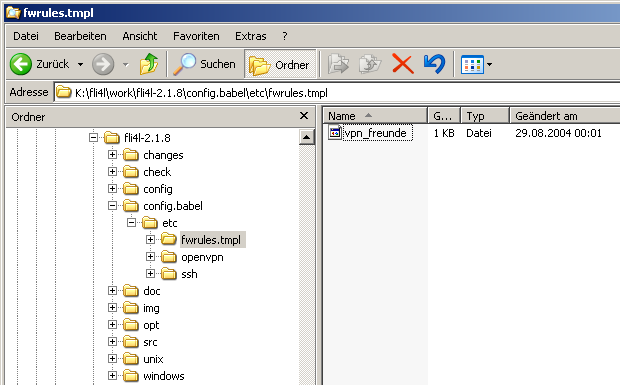
\includegraphics[width=0.9\columnwidth]{etc_fwrules_tmpl_dir}
  \caption{Verzeichnisstruktur fli4l}
  \label{fig:etc_fwrules_tmpl_dir}
\end{figure}

Es ist auch möglich, dass Sie eigene Schablonen anlegen oder dass
Pakete ihre eigenen Schablonen mitbringen. Um eine eigene
Schablone anzulegen, muss lediglich eine Datei mit den Namen der
Schablone erstellt und die entsprechenden Regeln dort
aufgenommen werden. Wenn Sie eine private Schablonendatei anlegen wollen,
erstellen Sie diese in dem Verzeichnis \verb+etc/fwrules.tmpl+ unterhalb Ihres
\texttt{config}-Verzeichnisses, so wie es die Abbildung
\ref{fig:etc_fwrules_tmpl_dir} zeigt. Wenn das Verzeichnis
\texttt{etc/fwrules.tmpl} unterhalb Ihres \texttt{config}-Verzeichnisses noch
nicht existiert, legen Sie bitte zuerst beide Verzeichnisse an. Alternativ
können Paket-Entwickler oder Benutzer, die Schablonen für mehr als eine
Konfiguration anlegen wollen, ihre Regeln direkt in das Verzeichnis
\texttt{opt/etc/fwrules.tmpl} ablegen. In dieses Verzeichnis kommen dann die
neuen Schablonen. Dabei gilt die Regel, dass die Schablonen im
\texttt{config}-Verzeichnis des Benutzers vorrangig behandelt werden.
Zum Schluss wird die Schablonendatei, die zum Lieferumfang von
fli4l gehört, ausgewertet. Sie können also Einträge in der fli4l-Schablonendatei
dadurch \glqq{}überschreiben\grqq{}, indem Sie eine
Schablonendatei mit dem Namen der zu überschreibenden Schablone in Ihrem
\texttt{config}-Verzeichnis anlegen.

Wenn Sie zum Beispiel die Schablone \fwmatch{vpn\_freunde} anlegen wollen, legen
Sie die Datei \texttt{vpn\_freunde} an. Das Template soll die Dienste
\protocol{ssh}, \protocol{smtp}, \protocol{dns} und \protocol{samba} enthalten.
Also schreiben Sie in die Datei \texttt{vpn\_freunde} Folgendes:

\begin{example}
\begin{verbatim}
    prot:tcp 22
    prot:tcp 25
    53
    prot:udp 137-138
    prot:tcp 139
    prot:tcp 445
\end{verbatim}
\end{example}

\noindent Wann immer Sie jetzt die Schablone \fwmatch{vpn\_freunde} benutzen,
werden daraus Regeln für alle darin aufgeführten Protokolle und Ports erzeugt.
\verb+PF_FORWARD_x='tmpl:vpn_freunde ACCEPT'+ etwa erstellt folgende
\fwchain{FORWARD}-Regeln:

\begin{example}
\begin{verbatim}
    prot:tcp 22 ACCEPT
    prot:tcp 25 ACCEPT
    53 ACCEPT
    prot:udp 137-138 ACCEPT
    prot:tcp 139 ACCEPT
    prot:tcp 445 ACCEPT
\end{verbatim}
\end{example}

\subsection{Die Konfiguration des Paketfilters}

Der Paketfilter wird im Wesentlichen durch vier Array-Variablen konfiguriert:

\begin{itemize}
  \item \var{PF\_INPUT\_\%} konfiguriert die \fwchain{INPUT}-Kette,
  \item \var{PF\_FORWARD\_\%} konfiguriert die \fwchain{FORWARD}-Kette,
  \item \var{PF\_OUTPUT\_\%} konfiguriert die \fwchain{OUTPUT}-Kette,
  \item \var{PF\_PREROUTING\_\%} konfiguriert die \fwchain{PREROUTING}-Kette und
  \item \var{PF\_POSTROUTING\_\%} konfiguriert die \fwchain{POSTROUTING}-Kette.
\end{itemize}

\configlabel{PF\_LOG\_LEVEL}{PFLOGLEVEL} Für alle folgenden Ketten
gilt die in \var{PF\_LOG\_LEVEL} vorgenommene Einstellung der
Protokoll-Stufe, deren Inhalt auf einen der folgenden Werte gesetzt werden
kann: \fwloglevel{debug}, \fwloglevel{info}, \fwloglevel{notice},
\fwloglevel{warning}, \fwloglevel{err}, \fwloglevel{crit}, \fwloglevel{alert},
\fwloglevel{emerg}.

\subsubsection{Die \fwchain{INPUT}-Kette}

Über die \fwchain{INPUT}-Kette wird konfiguriert, wer auf den Router zugreifen
darf. Trifft keine der Regeln der \fwchain{INPUT}-Kette zu, bestimmt die
Standard-Aktion, was mit dem Paket passieren soll, und die Protokoll-Variable
bestimmt, ob es bei einer Ablehnung ins System-Protokoll geschrieben werden soll.

Bei den verwendeten Parametern gibt es die folgenden Einschränkungen:
\begin{itemize}
  \item Es können nur \fwaction{ACCEPT}, \fwaction{DROP} und \fwaction{REJECT}
    als Aktion angegeben werden.
  \item Bei einer Schnittstellen-Einschränkung kann man nur die
    Eingangsschnittstelle einschränken.
\end{itemize}

\begin{description}
\config{PF\_INPUT\_POLICY}{PF\_INPUT\_POLICY}{PFINPUTPOLICY}
Diese Variable beschreibt die Standard-Aktion, die angewandt wird,
wenn keine der anderen Regeln zutrifft. Möglich sind:

\begin{itemize}
\item \fwaction{ACCEPT} (nicht empfohlen)
\item \fwaction{REJECT}
\item \fwaction{DROP} (nicht empfohlen)
\end{itemize}

\config{PF\_INPUT\_ACCEPT\_DEF}{PF\_INPUT\_ACCEPT\_DEF}{PFINPUTACCEPTDEF}
Steht diese Variable auf `yes', werden Standard-Regeln generiert, die
für ein korrektes Funktionieren des Routers notwendig
sind. Standardmäßig sollte man hier `yes' eintragen.

Möchte man das Verhalten komplett selbst definieren, kann man
hier `no' eintragen, muss dann jedoch alle Regeln selbst definieren.
Eine zum Standardverhalten äquivalente Konfiguration würde wie folgt
aussehen (die Beschreibung der Liste für benutzerdefinierte Ketten erfolgt
\jump{sec:userlists}{hier}):

\begin{example}
{\footnotesize
\begin{verbatim}
    PF_INPUT_ACCEPT_DEF='no'
    #
    # limit ICMP echo requests - use a separate chain
    #
    PF_USR_CHAIN_N='1'
    PF_USR_CHAIN_1_NAME='usr-in-icmp'
    PF_USR_CHAIN_1_RULE_N='2'
    PF_USR_CHAIN_1_RULE_1='prot:icmp:echo-request length:0-150 limit:1/second:5 ACCEPT'
    PF_USR_CHAIN_1_RULE_2='state:RELATED ACCEPT'

    PF_INPUT_N='4'
    PF_INPUT_1='prot:icmp usr-in-icmp'
    PF_INPUT_2='state:ESTABLISHED,RELATED ACCEPT'
    PF_INPUT_3='if:lo:any ACCEPT'
    PF_INPUT_4='state:NEW 127.0.0.1 DROP BIDIRECTIONAL'
\end{verbatim}}
\end{example}

Die erste Regel verzweigt zur ratenlimitierenden ``usr-in-icmp''-Kette.
Die zweite Regel akzeptiert nur solche Pakete, die zu bestehenden Verbindungen
gehören (also Paketen, die entweder den Zustand \fwpktstate{ESTABLISHED} oder
\fwpktstate{RELATED} besitzen), und die dritte erlaubt lokale Kommunikation
(\verb+if:lo:any ACCEPT+). Die vierte filtert Pakete heraus,
die behaupten, lokale Kommunikation zu sein, aber nicht bereits von
der vorherigen Regel akzeptiert wurden.

Arbeitet man mit OpenVPN, muss man die Regeln
noch ergänzen, um die von diesen Paketen verwendeteten Ketten
einzubinden.

\begin{example}
\begin{verbatim}
    PF_INPUT_N='5'
    ...
    PF_INPUT_5='ovpn-chain'
\end{verbatim}
\end{example}

\config{PF\_INPUT\_LOG}{PF\_INPUT\_LOG}{PFINPUTLOG}
Definiert, ob abgelehnte Pakete vom Kernel protokolliert werden sollen.
Dabei können die Meldungen durch Aktivierung von \var{OPT\_KLOGD} über den
syslog-Dämon entsprechend der Konfiguration ausgegeben werden.

\config{PF\_INPUT\_LOG\_LIMIT}{PF\_INPUT\_LOG\_LIMIT}{PFINPUTLOGLIMIT}
Definiert, wie häufig Log-Einträge generiert werden. Die Häufigkeit
wird analog zur Limit-Einschränkung als \emph{n/Zeiteinheit} mit Bursts
beschrieben, also z.\,B. \texttt{3/minute:5}. Ist dieser Eintrag leer, wird der
Standardwert \texttt{1/second:5} verwendet; enhält er \texttt{none}, wird keine
Limitierung durchgeführt.

\configlabel{PF\_INPUT\_UDP\_REJ\_LIMIT}{PFINPUTUDPREJLIMIT}
\config{PF\_INPUT\_REJ\_LIMIT PF\_INPUT\_UDP\_REJ\_LIMIT}{PF\_INPUT\_REJ\_LIMIT}{PFINPUTREJLIMIT}
Definiert, wie häufig bei einer Ablehnung eines hereinkommenden Paketes
auch ein entsprechendes \fwaction{REJECT}-Paket generiert wird. Die Häufigkeit
wird analog zur Limit-Einschränkung als \emph{n/Zeiteinheit} mit Bursts
beschrieben, also z.\,B. \texttt{3/minute:5}. Ist das Limit überschritten, wird
das Paket einfach ignoriert (\fwaction{DROP}). Ist dieser Eintrag leer, wird
der Standardwert \texttt{1/second:5} verwendet; enhält er \texttt{none}, wird
keine Limitierung durchgeführt.

\config{PF\_INPUT\_ICMP\_ECHO\_REQ\_LIMIT}{PF\_INPUT\_ICMP\_ECHO\_REQ\_LIMIT}{PFINPUTICMPECHOREQLIMIT}
Definiert, wie häufig auf eine ICMP-Echo-Anfrage reagiert werden soll.
Die Häufigkeit wird analog zur Limit-Einschränkung als \emph{n/Zeitein-heit}
mit Bursts beschrieben, also z.\,B. \texttt{/minute:5}. Ist das
Limit überschritten, wird das Paket einfach ignoriert (\fwaction{DROP}). Ist
dieser Eintrag leer, wird der Standardwert \texttt{1/second:5} verwendet;
enhält er \texttt{none}, wird keine Limitierung durchgeführt.

\config{PF\_INPUT\_ICMP\_ECHO\_REQ\_SIZE}{PF\_INPUT\_ICMP\_ECHO\_REQ\_SIZE}{PFINPUTICMPECHOREQSIZE}
Definiert, wie groß eine empfangene ICMP-Echo-Anfrage sein darf (in Bytes). In
dieser Angabe sind neben den ``Nutzdaten'' auch die Paket-Header mit zu
berücksichtigen. Der Standard-Wert liegt bei 150 Bytes.

\configlabel{PF\_INPUT\_x}{PFINPUTx}
\configlabel{PF\_INPUT\_x\_COMMENT}{PFINPUTxCOMMENT}
\config{PF\_INPUT\_N PF\_INPUT\_x PF\_INPUT\_x\_COMMENT}{PF\_INPUT\_N}{PFINPUTN}
Liste der Regeln, die beschreiben, welche Pakete vom Router angenommen
bzw. verworfen werden.
\end{description}

\subsubsection{Die \fwchain{FORWARD}-Kette}

Über die \fwchain{FORWARD}-Kette wird konfiguriert, welche Pakete vom Router
weitergeleitet werden. Trifft keine der Regeln der \fwchain{FORWARD}-Kette zu,
bestimmt die Standard-Aktion, was mit dem Paket passieren soll,und die
Protokoll-Variable bestimmt, ob es bei einer Ablehnung ins System-Protokoll
geschrieben werden soll.

Bei den verwendeten Parametern gibt es die Einschränkung, dass nur
\fwaction{ACCEPT}, \fwaction{DROP} und \fwaction{REJECT} als Aktion angegeben
werden können.

\begin{description}
\config{PF\_FORWARD\_POLICY}{PF\_FORWARD\_POLICY}{PFFORWARDPOLICY}
Diese Variable beschreibt die Standard-Aktion, die angewandt wird,
wenn keine der anderen Regeln zutrifft. Möglich sind:

\begin{itemize}
\item \fwaction{ACCEPT}
\item \fwaction{REJECT}
\item \fwaction{DROP}
\end{itemize}

\config{PF\_FORWARD\_ACCEPT\_DEF}{PF\_FORWARD\_ACCEPT\_DEF}{PFFORWARDACCEPTDEF}
Bestimmt, ob der Router Pakete akzeptiert, die zu bestehenden
Verbindungen gehören. Steht diese Variable auf `yes', generiert fli4l
automatisch eine Regel, die Pakete mit dem entsprechenden Zustand
akzeptiert:

\verb+'state:ESTABLISHED,RELATED ACCEPT'+,

weiterhin eine Regel, die Pakete mit unbekanntem Zustand verwirft:

\verb+'state:INVALID DROP'+.

und schließlich eine Regel, die Pakete mit gefälschten IP-Adressen verwirft:

\verb+'state:NEW 127.0.0.1 DROP BIDIRECTIONAL'+.

Zusätzlich generieren die
anderen Subsysteme auch noch Standardregeln~-- eine Konfiguration ohne
Standardregeln mit Portweiterleitung und OpenVPN würde mindestens
folgende Regeln enthalten:

\begin{example}
\begin{verbatim}
    PF_FORWARD_ACCEPT_DEF='no'
    PF_FORWARD_N='5'
    PF_FORWARD_1='state:ESTABLISHED,RELATED ACCEPT'
    PF_FORWARD_2='state:INVALID DROP'
    PF_FORWARD_3='state:NEW 127.0.0.1 DROP BIDIRECTIONAL'
    PF_FORWARD_4='pfwaccess-chain'
    PF_FORWARD_5='ovpn-chain'
\end{verbatim}
\end{example}

\config{PF\_FORWARD\_LOG}{PF\_FORWARD\_LOG}{PFFORWARDLOG}
Definiert, ob abgelehnte Pakete vom Kernel protokolliert werden sollen.
Dabei können die Meldungen durch Aktivierung von \var{OPT\_KLOGD} über den
syslog-Dämon entsprechend der Konfiguration ausgegeben werden.

\config{PF\_FORWARD\_LOG\_LIMIT}{PF\_FORWARD\_LOG\_LIMIT}{PFFORWARDLOGLIMIT}
Definiert, wie häufig Log-Einträge generiert werden. Die Häufigkeit
wird analog zur Limit-Einschränkung als \emph{n/Zeiteinheit} mit Bursts
beschrieben, also z.\,B. \texttt{3/minute:5}. Ist dieser Eintrag leer, wird der
Standardwert \texttt{1/second:5} verwendet; enhält er \texttt{none}, wird keine
Limitierung durchgeführt.

\configlabel{PF\_FORWARD\_UDP\_REJ\_LIMIT}{PFFORWARDUDPREJLIMIT}
\config{PF\_FORWARD\_REJ\_LIMIT PF\_FORWARD\_UDP\_REJ\_LIMIT}{PF\_FORWARD\_REJ\_LIMIT}{PFFORWARDREJLIMIT}
Definiert, wie häufig bei einer Ablehnung eines hereinkommenden Paketes
auch ein entsprechendes \fwaction{REJECT}-Paket generiert wird. Die Häufigkeit
wird analog zur Limit-Einschränkung als \emph{n/Zeiteinheit} mit Bursts
beschrieben, also z.\,B. \texttt{3/minute:5}. Ist das Limit überschritten, wird
das Paket einfach ignoriert (\fwaction{DROP}). Ist dieser Eintrag leer, wird
der Standardwert \texttt{1/second:5} verwendet; enhält er \texttt{none}, wird
keine Limitierung durchgeführt.

\configlabel{PF\_FORWARD\_x}{PFFORWARDx}
\configlabel{PF\_FORWARD\_x\_COMMENT}{PFFORWARDxCOMMENT}
\config{PF\_FORWARD\_N PF\_FORWARD\_x PF\_FORWARD\_x\_COMMENT}{PF\_FORWARD\_N}{PFFORWARDN}
Liste der Regeln, die beschreiben, welche Pakete vom Router
weitergeleitet bzw. verworfen werden.
\end{description}

\subsubsection{Die \fwchain{OUTPUT}-Kette}

Über die \fwchain{OUTPUT}-Kette wird konfiguriert, worauf der Router selbst
zugreifen darf. Trifft keine der Regeln der \fwchain{OUTPUT}-Kette zu, bestimmt
die Standard-Aktion, was mit dem Paket passieren soll, und die
Protokoll-Variable bestimmt, ob es bei einer Ablehnung ins System-Protokoll
geschrieben werden soll.

Bei den verwendeten Parametern gibt es die folgenden Einschränkungen:
\begin{itemize}
  \item Es können nur \fwaction{ACCEPT}, \fwaction{DROP} und \fwaction{REJECT}
    als Aktion angegeben werden.
  \item Bei einer Schnittstellen-Einschränkung kann man nur die
    Ausgangsschnittstelle einschränken.
\end{itemize}

\begin{description}
\config{PF\_OUTPUT\_POLICY}{PF\_OUTPUT\_POLICY}{PFOUTPUTPOLICY}
Diese Variable beschreibt die Standard-Aktion, die angewandt wird,
wenn keine der anderen Regeln zutrifft. Möglich sind:

\begin{itemize}
\item \fwaction{ACCEPT}
\item \fwaction{REJECT}
\item \fwaction{DROP}
\end{itemize}

\config{PF\_OUTPUT\_ACCEPT\_DEF}{PF\_OUTPUT\_ACCEPT\_DEF}{PFOUTPUTACCEPTDEF}
Steht diese Variable auf `yes', werden Standard-Regeln generiert, die
für ein korrektes Funktionieren des Routers notwendig
sind. Standardmäßig sollte man hier `yes' eintragen.

Möchte man das Verhalten komplett selbst definieren, kann man
hier `no' eintragen, muss dann jedoch alle Regeln selbst definieren.
Eine zum Standardverhalten äquivalente Konfiguration würde wie folgt
aussehen:

\begin{example}
{\footnotesize
\begin{verbatim}
    PF_OUTPUT_ACCEPT_DEF='no'

    PF_OUTPUT_N='1'
    PF_OUTPUT_1='state:ESTABLISHED,RELATED ACCEPT'
\end{verbatim}}
\end{example}

Die erste (und einzige) Regel akzeptiert nur solche Pakete, die zu bestehenden
Verbindungen gehören (also Paketen, die entweder den Zustand
\fwpktstate{ESTABLISHED} oder \fwpktstate{RELATED} besitzen).

\config{PF\_OUTPUT\_LOG}{PF\_OUTPUT\_LOG}{PFOUTPUTLOG}
Definiert, ob abgelehnte Pakete vom Kernel protokolliert werden sollen.
Dabei können die Meldungen durch Aktivierung von \var{OPT\_KLOGD} über den
syslog-Dämon entsprechend der Konfiguration ausgegeben werden.

\config{PF\_OUTPUT\_LOG\_LIMIT}{PF\_OUTPUT\_LOG\_LIMIT}{PFOUTPUTLOGLIMIT}
Definiert, wie häufig Log-Einträge generiert werden. Die Häufigkeit
wird analog zur Limit-Einschränkung als \emph{n/Zeiteinheit} mit Bursts
beschrieben, also z.\,B. \texttt{3/minute:5}. Ist dieser Eintrag leer, wird der
Standardwert \texttt{1/second:5} verwendet; enhält er \texttt{none}, wird keine
Limitierung durchgeführt.

\configlabel{PF\_OUTPUT\_UDP\_REJ\_LIMIT}{PFOUTPUTUDPREJLIMIT}
\config{PF\_OUTPUT\_REJ\_LIMIT PF\_OUTPUT\_UDP\_REJ\_LIMIT}{PF\_OUTPUT\_REJ\_LIMIT}{PFOUTPUTREJLIMIT}
Definiert, wie häufig bei einer Ablehnung eines hereinkommenden Paketes
auch ein entsprechendes \fwaction{REJECT}-Paket generiert wird. Die Häufigkeit
wird analog zur Limit-Einschränkung als \emph{n/Zeiteinheit} mit Bursts
beschrieben, also z.\,B. \texttt{3/minute:5}. Ist das Limit überschritten, wird
das Paket einfach ignoriert (\fwaction{DROP}). Ist dieser Eintrag leer, wird
der Standardwert \texttt{1/second:5} verwendet; enhält er \texttt{none}, wird
keine Limitierung durchgeführt.

\configlabel{PF\_OUTPUT\_x}{PFOUTPUTx}
\configlabel{PF\_OUTPUT\_x\_COMMENT}{PFOUTPUTxCOMMENT}
\config{PF\_OUTPUT\_N PF\_OUTPUT\_x PF\_OUTPUT\_x\_COMMENT}{PF\_OUTPUT\_N}{PFOUTPUTN}
Liste der Regeln, die beschreiben, welche Pakete vom Router versandt
bzw. verworfen werden.
\end{description}

\marklabel{sec:userlists}{\subsubsection{Benutzerdefinierte Listen}}

Aus verschiedenen Gründen besteht manchmal der Bedarf, eigene Ketten
anzulegen und dort die Pakete genauer zu filtern. Diese Ketten kann
man mittels \var{PF\_USR\_CHAIN\_\%} definieren und mit Regeln füllen. Die
Namen der Ketten müssen dabei mit \emph{usr-} beginnen und können nach ihrer
Definition überall in der \fwchain{INPUT}- oder \fwchain{FORWARD}-Kette statt
einer Aktion eingesetzt werden. Als Beispiel soll hier die bereits vorher
verwendete ICMP-Filterkette dienen:

\begin{example}
{\footnotesize
\begin{verbatim}
    PF_USR_CHAIN_N='1'
    #
    # create usr-in-icmp
    #
    PF_USR_CHAIN_1_NAME='usr-in-icmp'
    #
    # add rule to usr-in-icmp
    #
    PF_USR_CHAIN_1_RULE_N='2'
    PF_USR_CHAIN_1_RULE_1='prot:icmp:echo-request length:0-150 limit:1/second:5 ACCEPT'
    PF_USR_CHAIN_1_RULE_2='state:RELATED ACCEPT'
    #
    # use chain in PF_INPUT
    #
    PF_INPUT_2='prot:icmp usr-in-icmp'
\end{verbatim}}
\end{example}

\begin{description}
\config{PF\_USR\_CHAIN\_N}{PF\_USR\_CHAIN\_N}{PFUSRCHAINN} Definiert die Anzahl
der benutzerdefinierten Ketten.

\config{PF\_USR\_CHAIN\_x\_NAME}{PF\_USR\_CHAIN\_x\_NAME}{PFUSRCHAINxNAME}
Definiert den Namen der benutzerdefinierten Kette. Dieser muss mit \emph{usr-}
beginnen.

\configlabel{PF\_USR\_CHAIN\_x\_RULE\_x}{PFUSRCHAINxRULEx}
\configlabel{PF\_USR\_CHAIN\_x\_RULE\_x\_COMMENT}{PFUSRCHAINxRULExCOMMENT}
\config{PF\_USR\_CHAIN\_x\_RULE\_N}{PF\_USR\_CHAIN\_x\_RULE\_N}{dummy0}
\config{PF\_USR\_CHAIN\_x\_RULE\_x}{PF\_USR\_CHAIN\_x\_RULE\_N}{dummy1}
\config{PF\_USR\_CHAIN\_x\_RULE\_x\_COMMENT}{PF\_USR\_CHAIN\_x\_RULE\_N}{PFUSRCHAINxRULEN}
Hier werden die Regeln definiert, die in die benutzerdefinierte Kette
eingefügt werden sollen. Es können alle Regeln verwendet werden, die
auch in einer \fwchain{FORWARD}-Kette verwendet werden könnten.
Sollte keine Regel der benutzerdefinierten Kette zutreffen, wird zur
Ausgangskette zurückgekehrt und mit der Regel nach der Verzweigung fortgefahren.
\end{description}

\subsubsection{Die NAT-Ketten (Network Address Translation)}

Pakete können vor und nach Routing-Entscheidungen noch manipuliert
werden. Sie können zum Beispiel eine neue Zieladresse erhalten, um an einen
anderen Rechner weitergeleitet zu werden (Portweiterleitung) oder eine
andere Quelladresse erhalten, um das hinter dem Router liegende
Netzwerk zu maskieren. Maskieren nutzt man beispielsweise, um ein privates Netz
über eine öffentliche IP ins Netz zu bringen oder in einem DMZ-Setup
die Struktur des lokalen Netzes vor den Rechnern in der DMZ zu
verbergen.

Die Konfiguration erfolgt über zwei Ketten, die \fwchain{PREROUTING}- und die
\fwchain{POSTROUTING}-Kette. Über die \fwchain{POSTROUTING}-Kette wird
konfiguriert, welche Pakete vom Router maskiert werden. Trifft keine der Regeln
der \fwchain{POSTROUTING}-Kette zu, werden die Pakete unmaskiert
weitergeleitet. 

Beim Maskieren gibt es zwei Varianten: eine für Netzwerk-Schnittstellen, die
bei der Einwahl erst eine IP-Adresse zugewiesen bekommen
(\fwaction{MASQUERADE}) und eine für Netzwerk-Schnittstellen mit statischer
IP-Adresse (\fwaction{SNAT}). \fwaction{SNAT} erwartet dabei zusätzlich die
IP-Adresse, die im Paket als Quelle eingetragen werden soll. Diese kann als
\begin{itemize}
\item IP-Adresse (Beispiel: \fwaction{SNAT:1.2.3.4}),
\item IP-Bereich (Beispiel: \fwaction{SNAT:1.2.3.4-1.2.3.10})
\item oder als symbolische Referenz (Beispiel:
\fwaction{SNAT:IP\_NET\_1\_IPADDR})
\end{itemize}
angegeben werden.

Sowohl bei \fwaction{SNAT} als auch bei \fwaction{MASQUERADE} kann schließlich
ein Port bzw. Portbereich angegeben werden, auf den der
Quellport abgebildet werden soll. Normalerweise ist das nicht nötig,
da der Kern die Ports allein auswählen kann. Es gibt aber
Anwendungen, die verlangen, dass der Quellport unverändert bleibt
(und somit ein 1:1-NAT erfordern) oder die ein PAT (Port Address Translation)
oder NAPT (Network Address and Port Translation) verbieten. Der Portbereich wird
einfach hinten angehängt, z.\,B. so:
\fwaction{SNAT:IP\_NET\_1\_IPADDR:4000-8000}.

Bei der \fwchain{POSTROUTING}-Kette können nur \fwaction{ACCEPT},
\fwaction{SNAT}, \fwaction{NETMAP} und \fwaction{MASQUERADE} als Aktionen
verwendet werden.

\begin{description}

\configlabel{PF\_POSTROUTING\_x}{PFPOSTROUTINGx}
\configlabel{PF\_POSTROUTING\_x\_COMMENT}{PFPOSTROUTINGxCOMMENT}
\config{PF\_POSTROUTING\_N PF\_POSTROUTING\_x PF\_POSTROUTING\_x\_COMMENT}{PF\_POSTROUTING\_N}{PFPOSTROUTINGN}
\mbox{}\newline
Eine Liste der Regeln, die beschreiben, welche Pakete vom Router maskiert
werden (bzw. unmaskiert weitergeleitet werden). Will man Pakete vom
Maskieren ausklammern, kann man eine ACCEPT-Regel für die
auszuklammernden Pakete der MASQUERADE-Regel voranstellen.

\end{description}

Über die \fwchain{PREROUTING}-Kette wird konfiguriert, welche Pakete an einen
anderen Rechner weitergeleitet werden sollen. Trifft keine der Regeln
der \fwchain{PREROUTING}-Kette zu, werden die Pakete unverändert
weiterbehandelt. Die Aktion \fwaction{DNAT} erwartet dabei die IP-Adresse, die
im Paket als Ziel eingetragen werden soll. Diese kann als
\begin{itemize}
\item IP-Adresse (Beispiel: \fwaction{DNAT:1.2.3.4}),
\item IP-Bereich (Beispiel: \fwaction{DNAT:1.2.3.4-1.2.3.10})
\item oder als Hostname (Beispiel: \fwaction{DNAT:@client1})
\end{itemize}
angegeben werden.

Schließlich kann noch ein Port bzw. Portbereich angegeben werden, auf den der
Zielport abgebildet werden soll. Das ist aber nur nötig, wenn der Port geändert
werden soll. Der Port bzw. Portbereich wird einfach hinten angehängt, z.\,B.
so:
\fwaction{DNAT:@server:21}.

\fwaction{REDIRECT} verhält sich wie \fwaction{DNAT}, nur dass die
Ziel-IP-Adresse immer auf die (primäre) IP-Adresse der Schnittstelle, auf der das
Paket hereinkam, gesetzt wird und damit das Paket lokal zugestellt wird. Dies
wird z.\,B. für transparente Proxys benötigt, siehe
\jump{OPTTRANSPROXY}{\var{OPT\_TRANSPROXY}}.

Will man eine Portweiterleitung auf Schnittstellen mit dynamischen Adressen
machen, weiß man zum Zeitpunkt der Konfiguration noch nicht, an welche IP die
Pakete gerichtet sein werden. Daher kann man in der \fwchain{PREROUTING}-Kette
\fwmatch{dynamic} als Platzhalter für die später zugewiesene IP verwenden, etwa
wie folgt:

\begin{example}
{\footnotesize
\begin{verbatim}
    'dynamic:80  DNAT:1.2.3.4'           # leite http-Pakete an die
                                         # IP-Adresse 1.2.3.4 weiter
    'prot:gre any dynamic DNAT:1.2.3.4'  # leite gre-Pakete (Teil des PPTP-
                                         # Protokolls) an die IP-Adresse
                                         # 1.2.3.4 weiter
\end{verbatim}}
\end{example}

Bei der \fwchain{PREROUTING}-Kette können nur \fwaction{ACCEPT},
\fwaction{DNAT}, \fwaction{NETMAP} und \fwaction{REDIRECT} als Aktionen
verwendet werden.

Für weitere Beispiele zur Portweiterleitung siehe den nächsten Abschnitt.

\begin{description}

\configlabel{PF\_PREROUTING\_x}{PFPREROUTINGx}
\configlabel{PF\_PREROUTING\_x\_COMMENT}{PFPREROUTINGxCOMMENT}
\config{PF\_PREROUTING\_N PF\_PREROUTING\_x PF\_PREROUTING\_x\_COMMENT}{PF\_PREROUTING\_N}{PFPREROUTINGN}
\mbox{}\newline
Eine Liste der Regeln, die beschreiben, welche Pakete vom Router an ein
anderes Ziel weitergeleitet werden sollen.

\end{description}

\subsection{Beispiele}

Im Folgenden sind einige Beispiele für die Paketfilter-Konfiguration angegeben.

\subsubsection{Die fli4l-Standardkonfiguration}

Die fli4l-Standardkonfiguration der Distribution sieht für die
\fwchain{INPUT}-Kette wie folgt aus:

\begin{example}
\begin{verbatim}
    PF_INPUT_POLICY='REJECT'
    PF_INPUT_ACCEPT_DEF='yes'
    PF_INPUT_LOG='no'
    PF_INPUT_N='1'
    PF_INPUT_1='IP_NET_1 ACCEPT'
\end{verbatim}
\end{example}

Damit erreichen wir, dass
\begin{itemize}
\item Rechner im lokalen Netzwerk auf den Router zugreifen dürfen\\
(\verb+PF_INPUT_1='IP_NET_1 ACCEPT'+),
\item lokale Kommunikation auf dem Router erlaubt ist
  (\verb+PF_INPUT_ACCEPT_DEF='yes'+),
\item Pakete, die zu vom Router aufgebauten Verbindungen gehören,
  akzeptiert werden \newline (\verb+PF_INPUT_ACCEPT_DEF='yes'+),
\item alles andere abgelehnt wird (\verb+PF_INPUT_POLICY='REJECT'+),
\item aber nicht ins System-Protokoll geschrieben wird
  (\verb+PF_INPUT_LOG='no'+).
\end{itemize}

Für die \fwchain{FORWARD}-Kette sieht das so ähnlich aus: Nur Pakete unseres
lokalen Netzes und Pakete, die zu Verbindungen gehören, die von
Rechnern im lokalen Netz aufgebaut wurden, sollen weitergeleitet
werden. Des Weiteren werden NetBIOS- und CIFS-Pakete verworfen.

\begin{example}
\begin{verbatim}
    PF_FORWARD_POLICY='REJECT'
    PF_FORWARD_ACCEPT_DEF='yes'
    PF_FORWARD_LOG='no'
    PF_FORWARD_N='2'
    PF_FORWARD_1='tmpl:samba DROP'
    PF_FORWARD_2='IP_NET_1 ACCEPT'
\end{verbatim}
\end{example}

Was man hier gut sieht, ist die Abhängigkeit von der Reihenfolge der
Regeln: \emph{Zuerst} werden NetBIOS-Pakete verworfen, und \emph{danach} werden
die Pakete des lokalen Netzes akzeptiert.

Nun kann das lokale Netz mit dem Router kommunizieren, seine Pakete
werden weitergeleitet, es fehlt nur noch das Maskieren, welches für
den Zugriff eines privaten Netzwerkes auf das Internet notwendig ist:

\begin{example}
\begin{verbatim}
    PF_POSTROUTING_N='1'
    PF_POSTROUTING_1='IP_NET_1 MASQUERADE'
\end{verbatim}
\end{example}

\subsubsection{Trusted Nets}

Wollen wir lokal mehrere Subnetze haben, die frei und unmaskiert
miteinander kommunizieren können, müssen wir dafür sorgen, dass Pakete
zwischen diesen Subnetzen nicht verworfen und auch nicht maskiert
werden. Dazu fügen wir einfach eine Regel hinzu oder modifizieren die vorhandene.

Angenommen, wir haben einen DSL-Zugang über PPPoE, und die beiden Subnetze sind
\var{IP\_NET\_1} (192.168.6.0/24) und \var{IP\_NET\_2} (192.168.7.0/24).
Dann würde die Konfiguration wie folgt aussehen:

\begin{example}
\begin{verbatim}
    PF_FORWARD_POLICY='REJECT'
    PF_FORWARD_ACCEPT_DEF='yes'
    PF_FORWARD_LOG='no'
    PF_FORWARD_N='4'
    PF_FORWARD_1='IP_NET_1 IP_NET_2 ACCEPT BIDIRECTIONAL'
    PF_FORWARD_2='tmpl:samba DROP'
    PF_FORWARD_3='IP_NET_1 ACCEPT'
    PF_FORWARD_4='IP_NET_2 ACCEPT'

    PF_POSTROUTING_N='3'
    PF_POSTROUTING_1='IP_NET_1 IP_NET_2 ACCEPT BIDIRECTIONAL'
    PF_POSTROUTING_2='IP_NET_1 MASQUERADE'
    PF_POSTROUTING_3='IP_NET_2 MASQUERADE'
\end{verbatim}
\end{example}

Regel eins sorgt jetzt dafür, dass Pakete zwichen den beiden
Subnetzen ohne weitere Prüfung weitergeleitet werden. Die Regeln drei und vier
sorgen dafür, dass beide Subnetze auch ins Internet kommen. Die erste Regel
der \fwchain{POSTROUTING}-Kette sorgt dafür, dass die Kommunikation zwischen
den Subnetzen unmaskiert erfolgt.

Alternativ könnten wir auch sagen, dass nur Pakete, die über die
\fwmatch{pppoe}-Schnittstelle hinausgehen, maskiert werden sollen:

\begin{example}
\begin{verbatim}
    PF_POSTROUTING_N='1'
    PF_POSTROUTING_1='if:any:pppoe MASQUERADE'
\end{verbatim}
\end{example}

Genauso hätte man die Filterung der Ports auch auf die
\fwmatch{pppoe}-Schnittstelle beschränken und die beiden Subnetze zu einem
zusammenfassen können, das würde dann wie folgt aussehen:

\begin{example}
\begin{verbatim}
    PF_FORWARD_POLICY='REJECT'
    PF_FORWARD_ACCEPT_DEF='yes'
    PF_FORWARD_LOG='no'
    PF_FORWARD_N='2'
    PF_FORWARD_1='if:any:pppoe tmpl:samba DROP'
    PF_FORWARD_2='192.168.6.0/23 ACCEPT'

    PF_POSTROUTING_N='1'
    PF_POSTROUTING_1='if:any:pppoe MASQUERADE'
\end{verbatim}
\end{example}

Pakete, die über die \fwmatch{pppoe}-Schnittstelle hinausgehen und die an die
\protocol{udp}-Ports 137-138 oder an die \protocol{tcp}-Ports 139 und 445
adressiert sind, werden verworfen (Regel~1), alle anderen Pakete, die aus dem
Subnetz 192.168.6.0/23 kommen, werden weitergeleitet (Regel~2).

\subsubsection{Route Network}

Fügen wir dem Ganzen noch ein Netzwerk 10.0.0.0/24 hinzu (z.\,B. ein
Dial-In-Netzwerk), mit dem wir unmaskiert kommunizieren wollen, wobei
Pakete an die \protocol{udp}-Ports 137-138 sowie an die \protocol{tcp}-Ports
139 und 445 verworfen werden sollen, dann würde das wie folgt aussehen:

\begin{example}
\begin{verbatim}
    PF_FORWARD_POLICY='REJECT'
    PF_FORWARD_ACCEPT_DEF='yes'
    PF_FORWARD_LOG='no'
    PF_FORWARD_N='4'
    PF_FORWARD_1='IP_NET_1 IP_NET_2 ACCEPT BIDIRECTIONAL'
    PF_FORWARD_2='tmpl:samba DROP'
    PF_FORWARD_3='192.168.6.0/23 ACCEPT'
    PF_FORWARD_4='10.0.0.0/24 ACCEPT'

    PF_POSTROUTING_N='2'
    PF_POSTROUTING_1='10.0.0.0/24 ACCEPT BIDIRECTIONAL'
    PF_POSTROUTING_2='192.168.6.0/23 MASQUERADE'
\end{verbatim}
\end{example}

\begin{itemize}
\item Regel~1 erlaubt die ungehinderte Kommunikation zwischen den Subnetzen
  \var{IP\_NET\_1} und \var{IP\_NET\_2}.
\item Regel~2 verwirft Pakete an die Samba-Ports.
\item Die Regeln 3 und 4 erlaubt die Weiterleitung von Paketen, die aus den
  Subnetzen 192.168.6.0/24, 192.168.7.0/24 und 10.0.0.0/24 kommen; die
  Rückrichtung wird von der Einstellung \verb+PF_FORWARD_ACCEPT_DEF='yes'+
  abgedeckt.
\item Regel~1 der \fwchain{POSTROUTING}-Kette sorgt dafür, dass Pakete in
das bzw. aus dem 10.0.0.0/24-Subnetz nicht maskiert werden.
\end{itemize}

Alternativ ginge auch:

\begin{example}
\begin{verbatim}
    PF_POSTROUTING_N='1'
    PF_POSTROUTING_1='if:any:pppoe MASQUERADE'
\end{verbatim}
\end{example}

Diese Regel besagt, dass nur Pakete, die über die \fwmatch{pppoe}-Schnittstelle
hinausgehen, maskiert werden.

\subsubsection{Blacklists, Whitelists}

Blacklists (ein Rechner in dieser Liste darf etwas nicht) und
Whitelists (ein Rechner in dieser Liste darf etwas) werden prinzipiell
ähnlich umgesetzt. Es werden Regeln geschrieben, die am Anfang sehr
speziell sind und nach hinten immer allgemeiner werden. Bei einer
Blacklist stehen am Anfang Regeln, die etwas verbieten und am Ende
Regeln, die allen bisher nicht erwähnten etwas erlauben. Bei einer
Whitelist ist es genau umgekehrt.

\emph{Beispiel~1:} Alle Rechner im Subnetz 192.168.6.0/24 außer Rechner 12
dürfen ins Internet, solange sie nicht mit den CIFS Ports 137-138
(\protocol{udp}), 139 und 445 (\protocol{tcp}) kommunizieren wollen:

\begin{example}
\begin{verbatim}
    PF_FORWARD_POLICY='REJECT'
    PF_FORWARD_ACCEPT_DEF='yes'
    PF_FORWARD_LOG='no'
    PF_FORWARD_N='3'
    PF_FORWARD_1='192.168.6.12 DROP'
    PF_FORWARD_2='tmpl:samba DROP'
    PF_FORWARD_3='192.168.6.0/23 ACCEPT'

    PF_POSTROUTING_N='1'
    PF_POSTROUTING_2='192.168.6.0/24 MASQUERADE'
\end{verbatim}
\end{example}

\emph{Beispiel~2:} Nur Rechner 12 darf ins Internet (aber nicht an die o.\,g.
Ports \ldots), alle anderen dürfen nur lokal mit einem anderen Subnetz
kommunizieren:

\begin{example}
\begin{verbatim}
    PF_FORWARD_POLICY='REJECT'
    PF_FORWARD_ACCEPT_DEF='yes'
    PF_FORWARD_LOG='no'
    PF_FORWARD_N='3'
    PF_FORWARD_1='192.168.6.0/24 192.168.7.0/24 ACCEPT BIDIRECTIONAL'
    PF_FORWARD_2='tmpl:samba DROP'
    PF_FORWARD_3='192.168.6.12 ACCEPT'

    PF_POSTROUTING_N='1'
    PF_POSTROUTING_1='if:any:pppoe MASQUERADE'
\end{verbatim}
\end{example}

\subsection{Standardkonfigurationen}

\subsubsection{Einfacher maskierender Router mit einem Netz dahinter}

\begin{example}
\begin{verbatim}
#
# Zugriff auf den Router
#
PF_INPUT_POLICY='REJECT'
PF_INPUT_ACCEPT_DEF='yes'
PF_INPUT_LOG='no'
PF_INPUT_N='1'
PF_INPUT_1='IP_NET_1 ACCEPT'   # alle Hosts im lokalen Netz dürfen
                               # auf den Router zugreifen

#
# Zugriff auf das ``Internet''
#
PF_FORWARD_POLICY='REJECT'
PF_FORWARD_ACCEPT_DEF='yes'
PF_FORWARD_LOG='no'

PF_FORWARD_N='2'
PF_FORWARD_1='tmpl:samba DROP' # Samba-Pakete, die das Netz
                               # verlassen wollen, werden verworfen
PF_FORWARD_2='IP_NET_1 ACCEPT' # alle anderen Pakete dürfen das
                               # lokale Netz verlassen

#
# Maskieren des lokalen Netzes
#
PF_POSTROUTING_N='1'
PF_POSTROUTING_1='IP_NET_1 MASQUERADE'  # maskiere Pakete, die das Subnetz
                                        # verlassen
\end{verbatim}
\end{example}

\subsubsection{Einfacher maskierender Router mit zwei Netzen dahinter}

\begin{example}
\begin{verbatim}
#
# Zugriff auf den Router
#
PF_INPUT_POLICY='REJECT'
PF_INPUT_ACCEPT_DEF='yes'
PF_INPUT_LOG='no'
PF_INPUT_N='2'
PF_INPUT_1='IP_NET_1 ACCEPT'   # alle Hosts im lokalen Netz dürfen
                               # auf den Router zugreifen
PF_INPUT_2='IP_NET_2 ACCEPT'   # alle Hosts im lokalen Netz dürfen
                               # auf den Router zugreifen

#
# Zugriff auf das ``Internet''
#
PF_FORWARD_POLICY='REJECT'
PF_FORWARD_ACCEPT_DEF='yes'
PF_FORWARD_LOG='no'

#
# Freie Kommunikation zwischen den Netzen
#
PF_FORWARD_N='4'
PF_FORWARD_1='IP_NET_1 IP_NET_2 ACCEPT BIDIRECTIONAL'
PF_FORWARD_2='tmpl:samba DROP' # Samba-Pakete, die das Netz
                               # verlassen wollen, werden verworfen
PF_FORWARD_3='IP_NET_1 ACCEPT' # alle anderen Pakete dürfen das
                               # lokale Netz verlassen
PF_FORWARD_4='IP_NET_2 ACCEPT' # alle anderen Pakete dürfen das
                               # lokale Netz verlassen

#
# Maskieren der lokalen Netze, unmaskierte Kommunikation zwischen den
# Netzen
#
PF_POSTROUTING_N='3'
PF_POSTROUTING_1'IP_NET_1 IP_NET_2 ACCEPT BIDIRECTIONAL'
PF_POSTROUTING_2='IP_NET_1 MASQUERADE'  # maskiere Pakete, die das Subnetz
                                        # verlassen
PF_POSTROUTING_3='IP_NET_2 MASQUERADE'  # maskiere Pakete, die das Subnetz
                                        # verlassen
\end{verbatim}
\end{example}

\subsubsection{Maskierender DSL-Router mit zwei Netzen dahinter und
SSH/HTTP-Zugriff aus dem Internet}

\begin{example}
\begin{verbatim}
#
# Zugriff auf den Router
#
PF_INPUT_POLICY='REJECT'
PF_INPUT_ACCEPT_DEF='yes'
PF_INPUT_LOG='no'
PF_INPUT_N='4'
PF_INPUT_1='IP_NET_1 ACCEPT'   # alle Hosts im lokalen Netz dürfen
                               # auf den Router zugreifen
PF_INPUT_2='IP_NET_2 ACCEPT'   # alle Hosts im lokalen Netz dürfen
                               # auf den Router zugreifen
PF_INPUT_3='tmpl:ssh ACCEPT'   # gestatte Zugriff auf SSH-Dienst
                               # von überall her
PF_INPUT_4='tmpl:http 1.2.3.4/24 ACCEPT'  # gestatte Rechner aus
                               # einem bestimmten Subnetz Zugriff
                               # auf HTTP-Dienst


#
# Zugriff auf das ``Internet''
#
PF_FORWARD_POLICY='REJECT'
PF_FORWARD_ACCEPT_DEF='yes'
PF_FORWARD_LOG='no'

#
# Keine Kommunikation zwischen den Netzen, beide Netze dürfen ins
# Internet, Samba-Pakete werden verworfen
#
PF_FORWARD_N='2'
PF_FORWARD_1='tmpl:samba if:any:pppoe DROP' # Samba-Pakete, die das Netz
                               # verlassen wollen, werden verworfen
PF_FORWARD_2='if:any:pppoe ACCEPT' # alle anderen Pakete dürfen das
                               # lokale Netz verlassen

#
# Maskieren der lokalen Netze, unmaskierte Kommunikation zwischen den
# Netzen
#
PF_POSTROUTING_N='1'
PF_POSTROUTING_1='if:any:pppoe MASQUERADE'  # maskiere Pakete, die das Subnetz
                                            # verlassen
\end{verbatim}
\end{example}

\subsubsection{Portweiterleitung}

Portweiterleitungen lassen sich mit den \fwchain{PREROUTING}-Regeln wie folgt
umsetzen (\verb+TARGET+ bezeichnet die ursprüngliche Zieladresse (optional) und
den ursprünglichen Zielport, \verb+NEW_TARGET+ bezeichnet die neue Zieladresse
und den neuen Zielport (optional), \verb+PROTOCOL+ bezeichnet das jeweilige
Protokoll):

\begin{example}
\begin{verbatim}
    TARGET='<port>'
    NEW_TARGET='<ip>'
    PROTOCOL='<proto>'
    PF_PREROUTING_x='prot:<proto> dynamic:<port> DNAT:<ip>'

    TARGET='<port1>-<port2>'
    NEW_TARGET='<ip>'
    PROTOCOL='<proto>'
    PF_PREROUTING_x='prot:<proto> dynamic:<port1>-<port2> DNAT:<ip>'

    TARGET='<ip>:<port-a>'
    NEW_TARGET='<ip>:<port-b>'
    PROTOCOL='<proto>'
    PF_PREROUTING_x='prot:<proto> any <ip>:<port-a> DNAT:<ip>:<port-b>'
\end{verbatim}
\end{example}

\subsubsection{Transparenter Proxy}
Will man bestimmte Zugriffe auf das Internet nur über einen lokalen Proxy
zulassen, kann man das mit Hilfe der \fwchain{PREROUTING}- und
\fwchain{POSTROUTING}-Ketten erzwingen, ohne dass der Client davon etwas merkt.
Prinzipiell sind dazu drei Schritte notwendig:

\begin{enumerate}
\item Anfragen an den HTTP-Port, die nicht vom Proxy kommen, an den
Proxy umleiten (\fwchain{PREROUTING}).
\item Die umgeleiteten Pakete so verändern, dass der Proxy denkt, sie
kommen vom Router, so dass er sie wieder dorthin zurückschickt
(\fwchain{POSTROUTING}).
\item Die Pakete durch die FORWARD-Kette durchlassen, sofern ein
Eintrag à la

\begin{example}
\begin{verbatim}
PF_FORWARD_x='IP_NET_1 ACCEPT'
\end{verbatim}
\end{example}

nicht existiert (\fwchain{FORWARD}).
\end{enumerate}

\emph{Beispiel~1:} Angenommen, wir haben nur ein Netz \var{IP\_NET\_1},
in dem auf einem Rechner namens \host{proxy} ein Squid-Proxy läuft, und
wollen den gesamten \protocol{http}-Datenverkehr über ihn leiten. Squid lauscht
auf Port 3128. Der Einfachheit halber beziehen wir uns via \host{@proxy} auf
den eingetragenen Host aus \verb+HOST_1_NAME='proxy'+ (vgl.
\jump{sec:domainkonfiguration}{Domainkonfiguration}).

Das Ganze würde wie folgt aussehen:

\begin{example}
\begin{verbatim}
...
  PF_PREROUTING_x='@proxy ACCEPT'
      # Pakete vom Proxy sollen nicht umgeleitet werden

  PF_PREROUTING_x='prot:tcp IP_NET_1 80 DNAT:@proxy:3128'
      # HTTP-Pakete aus IP_NET_1 mit einem beliebigen Ziel werden
      # umgeleitet nach @proxy, Port 3128

  PF_POSTROUTING_x='any @proxy:3128 SNAT:IP_NET_1_IPADDR'
      # alle Pakete an den Proxy-Port 3128 so umschreiben, als wären sie
      # vom fli4l (IP_NET_1_IPADDR)

  PF_FORWARD_x='prot:tcp @proxy 80 ACCEPT'
      # HTTP-Pakete vom Proxy durch die FORWARD-Kette durchlassen (wenn nötig)
...
\end{verbatim}
\end{example}

Gibt es mehrere Netze oder potentielle Konflikte mit anderen
Portweiterleitungen (die ja auch nichts anderes sind als
\fwaction{DNAT}-Regeln), muss man die Regeln vielleicht noch etwas enger
formulieren.

\emph{Beispiel~2:} Unser Proxy namens \host{proxy} steht in \var{IP\_NET\_1},
lauscht auf Port 3128 und soll nur für Clients aus \var{IP\_NET\_1} wirksam
werden. \var{IP\_NET\_1} ist über \var{IP\_NET\_1\_DEV} erreichbar. Pakete aus
weiteren Netzen sollen nicht berücksichtigt werden.

\begin{example}
\begin{verbatim}
...
  PF_PREROUTING_x='if:IP_NET_1_DEV:any !@proxy 80 DNAT:@proxy:3128'
      # Anfragen an den HTTP-Port, die nicht vom Proxy, aber über eine
      # interne Schnittstelle (IP_NET_1_DEV) kommen, an den Proxy-Port umleiten.
      # An dieser Stelle ist es wichtig, mit if:IP_NET_1_DEV:any zu
      # überprüfen, ob die Pakete von innen kommen, da sonst auch Pakete von
      # außen umgeleitet würden (Sicherheitslücke!).

  PF_POSTROUTING_x='prot:tcp IP_NET_1 @proxy:3128 SNAT:IP_NET_1_IPADDR'
      # HTTP-Pakete die aus IP_NET_1 stammen und für den Proxy-Port 3128
      # gedacht sind, so umschreiben, als wären sie vom fli4l (IP_NET_1_IPADDR)

  PF_FORWARD_x='prot:tcp @proxy 80 ACCEPT'
      # HTTP-Pakete vom Proxy durch die FORWARD-Kette durchlassen (wenn nötig)
...
\end{verbatim}
\end{example}

\emph{Beispiel~3:} Um sich das Leben etwas zu erleichtern und die Regeln
kürzer zu gestalten, kann man auch Templates einsetzen (vgl.
\jump{sec:templates}{Templates im Paketfilter}). Zweckmäßig ist an dieser
Stelle das \fwmatch{tmpl:http}, das in \fwmatch{prot:tcp any any:80}
übersetzt wird. So wird z.\,B. aus \fwmatch{tmpl:http IP\_NET\_1 DNAT:@proxy:3128}
dann \fwmatch{prot:tcp IP\_NET\_1 80 DNAT:@proxy:3128}.

Sowohl \var{IP\_NET\_1} als auch \var{IP\_NET\_2} sollen transparent über den
Proxy umgeleitet werden. Damit ließe sich vereinfacht auch schreiben:

\begin{example}
\begin{verbatim}
...
  PF_PREROUTING_x='tmpl:http @proxy   ACCEPT'
      # HTTP-Pakete vom Proxy sollen nicht umgeleitet werden

  PF_PREROUTING_x='tmpl:http IP_NET_1 DNAT:@proxy:3128'
      # HTTP-Pakete aus IP_NET_1 sollen umgeleitet werden

  PF_PREROUTING_x='tmpl:http IP_NET_2 DNAT:@proxy:3128'
      # HTTP-Pakete aus IP_NET_2 sollen umgeleitet werden

  PF_POSTROUTING_x='IP_NET_1 @proxy:3128 SNAT:IP_NET_1_IPADDR'
  PF_POSTROUTING_x='IP_NET_2 @proxy:3128 SNAT:IP_NET_2_IPADDR'

  PF_FORWARD_x='tmpl:http @proxy ACCEPT'
...
\end{verbatim}
\end{example}

Und so ließe sich das endlos fortsetzen \ldots

\marklabel{sec:dmz}{\subsection{DMZ~-- Demilitarisierte Zone}}

fli4l gestattet auch den Aufbau einer DMZ. 
Hier sei erstmal auf das Wiki verwiesen.
https://ssl.nettworks.org/wiki

\marklabel{sec:masqueradingmodule}{\subsection{Conntrack-Helfer}}

  Die Verwendung von IP-Masquerading\index{Masquerading}
  hat zwar den Vorteil, dass mehrere Rechner im LAN über eine
  einzige offizielle IP-Adresse geroutet werden kann, es gibt aber
  auch Nachteile, die man in Kauf nehmen muss.

  Ein großes Problem ist zum Beispiel, dass kein Rechner von außen
  von sich aus eine Verbindung zu einem Rechner aufnehmen kann.
  Das ist zwar aus Sicherheitsgründen eigentlich durchaus
  erwünscht, aber bestimmte Protokolle funktionieren nicht mehr,
  weil sie einen Verbindungsaufbau von außen einfach erfordern.

  Ein klassisches Beispiel ist FTP. Neben dem Kommunikationskanal,
  auf dem Befehle und Antworten ausgetauscht werden, wird ein
  weiterer Kanal (in Form eines IP-Ports) verwendet, um die
  eigentlichen Nutzdaten zu versenden. fli4l verwendet dafür
  bestimmte Conntrack-Helfer, um solche zusätzlichen Ports, die
  verwendet werden, ad hoc dann freizuschalten und an den internen
  Rechner weiterzuleiten, wenn sie benötigt werden. Dabei
  ``horcht'' der Conntrack-Helfer in den Datenstrom, um zu
  erkennen, wann ein zusätzlicher Port benötigt wird.

  Typische Anwendungen für Conntrack-Helfer sind
  Chat-Protokolle und Spiele im Internet.

  Ein solcher Conntrack-Helfer wird über Regeln in zwei speziellen Arrays
  aktiviert. Das Array \var{PF\_PREROUTING\_CT\_\%} enthält Helfer-Zuordnungen
  zu Paketen, die von außen kommen, das Array \var{PF\_OUTPUT\_CT\_\%}
  enthält Helfer-Zuordnungen zu Paketen, die auf dem Router generiert werden.
  Einige Beispiele aus der Praxis sollen dies verdeutlichen.
  
  \emph{Beispiel 1:} Soll aktives FTP aus dem LAN erlaubt werden, ist das
  aus der Sicht des Routers eine Verbindung von außerhalb, somit
  muss ein Eintrag in \var{PF\_PREROUTING\_CT\_\%} vorgenommen werden:
  
\begin{example}
\begin{verbatim}
    PF_PREROUTING_CT_N='1'
    PF_PREROUTING_CT_1='tmpl:ftp IP_NET_1 HELPER:ftp'
\end{verbatim}
\end{example}

  Damit wird für alle TCP-Verbindungen aus dem lokalen Netz (\var{IP\_NET\_1})
  zu irgendeiner anderen Adresse an Port 21 (dies ist der \protocol{ftp}-Port)
  das \protocol{ftp}-Hilfsmodul geladen. Dieses Modul erlaubt dann im Laufe
  der Verbindung, dass der FTP-Server zurück zum Client eine Datenverbindung
  aufbauen kann, indem temporär ein ``Loch'' in der Firewall aufgemacht wird.

  \emph{Beispiel 2:} Soll passives FTP für einen FTP-Server im LAN ermöglicht
  werden (dabei wird die Datenverbindung von außen nach innen aufgebaut, so
  dass auch hier kurzfristig ein Loch in der Firewall geöffnet werden muss),
  ist dies ebenfalls aus der Sicht des Router eine Verbindung von außerhalb des
  Routers. Hier sieht die Regel folgendermaßen aus:

\begin{example}
\begin{verbatim}
    PF_PREROUTING_CT_N='1'
    PF_PREROUTING_CT_1='tmpl:ftp any dynamic HELPER:ftp'
\end{verbatim}
\end{example}

  Mit dieser Regel wird ausgedrückt, dass alle FTP-Verbindungen, die an die
  dynamische Adresse des Routers gesandt werden, mit dem FTP-Conntrack-Helfer
  assoziiert werden. Hier wurde \fwmatch{dynamic} verwendet, da angenommen
  wird, dass der Router für die Einwahl ins Internet verantwortlich ist und
  somit eine externe IP-Adresse besitzt. Falls der Router eine Einwahl via
  DSL durchführt, kann man die Regel auch so schreiben:
  
\begin{example}
\begin{verbatim}
    PF_PREROUTING_CT_N='1'
    PF_PREROUTING_CT_1='tmpl:ftp if:pppoe:any HELPER:ftp'
\end{verbatim}
\end{example}

  Mit dieser Regel wird ausgedrückt, dass alle FTP-Verbindungen, die von der
  DSL-Schnitt\-stelle (\fwmatch{pppoe}) kommen, mit dem FTP-Conntrack-Helfer
  assoziiert werden.

  Falls der Router sich nicht einwählt, sondern z.\,B.
  hinter einem anderen Router (Fritz!Box, Kabelmodem etc.) hängt, so kann die
  folgende Regel verwendet werden:

\begin{example}
\begin{verbatim}
    PF_PREROUTING_CT_N='1'
    PF_PREROUTING_CT_1='tmpl:ftp if:IP_NET_2_DEV:any HELPER:ftp'
\end{verbatim}
\end{example}

  Dabei wird im Beispiel angenommen, dass die Verbindung zum anderen Router
  über die Schnittstelle durchgeführt wird, die dem zweiten Subnetz zugeordnet
  ist (\var{IP\_NET\_2\_DEV}).
  
  Zu beachten ist, dass natürlich \emph{zusätzlich} eine entsprechende
  Konfiguration der \fwchain{FORWARD}-Kette nötig ist, um die FTP-Pakete auch
  tatsächlich weiterzuleiten. Eine typische Regel wäre etwa
  
\begin{example}
\begin{verbatim}
    PF_PREROUTING_1='tmpl:ftp any dynamic DNAT:@ftpserver'
\end{verbatim}
\end{example}

  wobei angenommen wird, dass der Host, auf dem das FTP-Serverprogramm läuft,
  den Namen \host{ftpserver} hat.

  \emph{Beispiel 3:} Schließlich muss auch, wenn man vom fli4l direkt aktives
  FTP benutzen möchte (etwa mit Hilfe des \protocol{ftp}-Programms aus dem
  \package{tools}-Paket), die Firewall dafür vorbereitet werden, diesmal in der
  \fwchain{OUTPUT}-Kette, die mit Hilfe des Arrays \var{PF\_OUTPUT\_CT\_\%}
  konfiguriert wird:
  
\begin{example}
\begin{verbatim}
    PF_OUTPUT_CT_N='1'
    PF_OUTPUT_CT_1='tmpl:ftp HELPER:ftp'
\end{verbatim}
\end{example}

  Diese Regel ist jedoch unnötig, falls \verb+FTP_PF_ENABLE_ACTIVE='yes'+
  benutzt wird -- siehe hierzu die Dokumentation des \protocol{ftp}-OPTs im
  \package{tools}-Paket.

  Es folgt eine Übersicht über die existierenden Conntrack-Helfer:

\begin{center}
    \begin{longtable}{|l|p{0.5\textwidth}|}
        \hline
        \multicolumn{1}{|l}{\textbf{Helfer}} &
        \multicolumn{1}{|l|}{\textbf{Erläuterung}} \\
        \hline
        \endhead
        \hline
        \endfoot
        \endlastfoot
            \index{ftp}\protocol{ftp}      & File Transfer Protocol\\
        \hline
            \index{h323}\protocol{h323}    & H.323 (Voice over IP)\\
        \hline
            \index{irc}\protocol{irc}      & Internet Relay Chat\\
        \hline
            \index{pptp}\protocol{pptp}    & PPTP Masquerading
                (Mit diesem Modul lässt sich mehr als ein PPTP-Client
                gleichzeitig hinter einem fli4l-Router betreiben.)\\
        \hline
            \index{sip}\protocol{sip}      & Session Initiation Protocol \\
        \hline
            \index{sane}\protocol{sane}    & SANE Network Procotol \\
        \hline
            \index{snmp}\protocol{snmp}    & Simple Network Management Protocol \\
        \hline
            \index{tftp}\protocol{tftp}    & Trivial File Transfer Protocol \\
        \hline
        \caption{Verfügbare Conntrack-Helfer im Paketfilter}\marklabel{fwrule:cthelpers}{}
    \end{longtable}
\end{center}

  Es folgt eine Übersicht der zu konfigurierenden Variablen:

\begin{description}

\config{PF\_PREROUTING\_CT\_ACCEPT\_DEF}{PF\_PREROUTING\_CT\_ACCEPT\_DEF}{PFPREROUTINGCTACCEPTDEF}
Steht diese Variable auf `yes', werden Standard-Regeln generiert, die
für ein korrektes Funktionieren des Routers notwendig
sind. Standardmäßig sollte man hier `yes' eintragen.

\configlabel{PF\_PREROUTING\_CT\_x}{PFPREROUTINGCTx}
\configlabel{PF\_PREROUTING\_CT\_x\_COMMENT}{PFPREROUTINGCTxCOMMENT}
\config{PF\_PREROUTING\_CT\_N PF\_PREROUTING\_CT\_x PF\_PREROUTING\_CT\_x\_COMMENT}{PF\_PREROUTING\_CT\_N}{PFPREROUTINGCTN}
Liste der Regeln, die beschreiben, welche eingehenden Pakete vom Router mit
Conntrack-Helfern verbunden werden.

\config{PF\_OUTPUT\_CT\_ACCEPT\_DEF}{PF\_OUTPUT\_CT\_ACCEPT\_DEF}{PFOUTPUTCTACCEPTDEF}
Steht diese Variable auf `yes', werden Standard-Regeln generiert, die
für ein korrektes Funktionieren des Routers notwendig
sind. Standardmäßig sollte man hier `yes' eintragen.

\configlabel{PF\_OUTPUT\_CT\_x}{PFOUTPUTCTx}
\configlabel{PF\_OUTPUT\_CT\_x\_COMMENT}{PFOUTPUTCTxCOMMENT}
\config{PF\_OUTPUT\_CT\_N PF\_OUTPUT\_CT\_x PF\_OUTPUT\_CT\_x\_COMMENT}{PF\_OUTPUT\_CT\_N}{PFOUTPUTCTN}
\mbox{}\\
Liste der Regeln, die beschreiben, welche auf dem Router generierten Pakete vom
Router mit Conntrack-Helfern verbunden werden.

\end{description}
